\begin{frame}
    \frametitle{Cyclus Simulation of historic U.S. nuclear fuel cycle}
        Reactor deployment data obtained from the Power Reactor Information System (PRIS) database \cite{peterson_unf_2017} for the 112 commercial nuclear reactors that have operated since 1968 was used to create a \textsc{Cyclus} \textbf{simulation of the U.S. nuclear fuel cycle}. 
        \begin{columns}
        \column[t]{5cm}
    \begin{figure}[htbp!]
      \begin{center}
        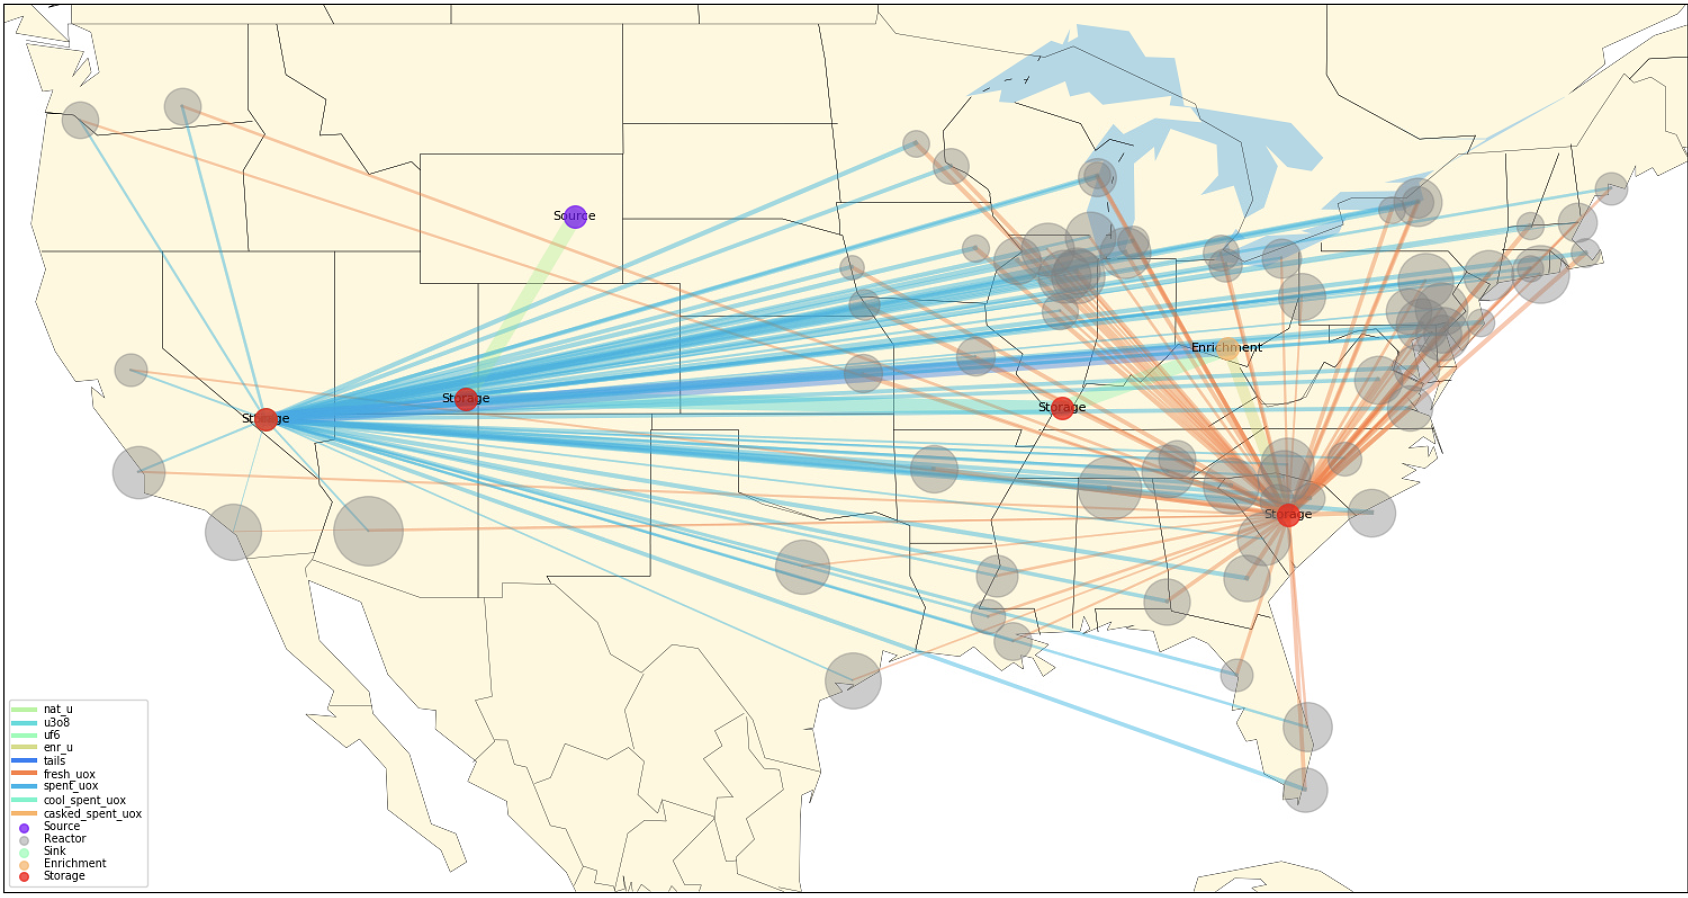
\includegraphics[height=3cm]{../figures/cycmap}
      \end{center}
            \caption{Cycmap of the historic Cyclus U.S nuclear fuel cycle simulation \cite{park_arfc/cycmap_2018}}
      \label{fig:cycmap}
    \end{figure}
    \column[t]{5cm}
    \textbf{Assumptions} 
    \begin{itemize}
    \item constant refueling time 
    \item constant reactor cycle time 
    \item single spent fuel depletion composition
    \end{itemize}
  \end{columns}
  \end{frame}
